% Preview source code

%% LyX 2.0.5.1 created this file.  For more info, see http://www.lyx.org/.
%% Do not edit unless you really know what you are doing.
\documentclass[english]{article}
\usepackage[T1]{fontenc}
\usepackage[latin9]{inputenc}
\usepackage{array}
\usepackage{float}
\usepackage{textcomp}
\usepackage{url}
\usepackage{multirow}
\usepackage{graphicx}
\usepackage{setspace}

\makeatletter

%%%%%%%%%%%%%%%%%%%%%%%%%%%%%% LyX specific LaTeX commands.
%% Because html converters don't know tabularnewline
\providecommand{\tabularnewline}{\\}

\makeatother

\usepackage{babel}
\begin{document}
\begin{center}
\pagenumbering{roman}
\par\end{center}

\begin{center}
\textbf{\Large{Construction of an Ecological Tool to Generate 2D Natural
and Urban Landscapes}}
\par\end{center}{\Large \par}

\medskip{}


\begin{center}
A Project Report Submitted
\par\end{center}

\begin{center}
in Partial Fulfillment of Requirements
\par\end{center}

\begin{center}
for the Degree of
\par\end{center}

\medskip{}


\begin{center}
\textbf{Bachelor of Technology}
\par\end{center}

\medskip{}


\begin{center}
By
\par\end{center}

\begin{center}
{\Large{Sonu Kumar Giri (P2009CS1043)}}\bigskip{}

\par\end{center}

\begin{center}

\includegraphics[scale=0.6]{logo}
\par\end{center}

\begin{center}
Department of Computer Science \& Engineering
\par\end{center}

\begin{center}
Indian Institute of Technology Ropar
\par\end{center}

\begin{center}
Rupnagar 140001, India
\par\end{center}

\begin{center}
May 2013
\par\end{center}

\begin{center}
{\LARGE{\newpage{}Abstract}}
\par\end{center}{\LARGE \par}

\bigskip{}


In landscape ecology synthetic 2D landscape generators can be used
in theoretical models to test ecological processes, models and uncertainty
in ecological data. Ecological studies using real data are restricted
by available data and the cost of acquiring new data meaning that
samples sizes tend to be small reducing the possibility of making
generalizations. Conclusions derived may thus be specific to a particular
area described by the limited data available. Studies that have a
large sample size tend to use simulated landscapes (e.g. Li et al.
2005). In this project we constructed a tool to generate synthetic
2D landscape with natural and urban landscapes. This tool generates
synthetic landscape with various features based on the input provided
by user. In this paper, we describe the algorithms used in the tool
to generate the landscapes, input parameters for the tool, results
obtained, and future improvements.

\medskip{}


Output obtained for a particular input parameter is presented. We
also describe the installation procedure for our tool on linux machines.
This tool is freely available and can be downloaded from github \url{( https://github.com/SonuGiriIITP/LandscapeSimGRASS_GIS ). }

\newpage{}

\begin{center}
{\LARGE{Acknowledgements}}
\par\end{center}{\LARGE \par}

\bigskip{}


I would like to express our sincere thanks to Indian Institute of
Technology, Ropar for providing us with the environment and resources
to carry out our project.

\medskip{}


Apart from the efforts of myself, the success of this project depends
largely on the encouragement and guidelines of many others. I take
this opportunity to express my profound gratitude and deep regards
to my mentors Dr. Lucy Bastin and Dr. Alex Lechner for their exemplary
guidance, monitoring and constant encouragement throughout the course
of this project.

\medskip{}


I am obliged to faculty of Computer Science at IIT Ropar, Dr. Apurva
Mudgal, Dr. Sudarshan Iyengar, Dr. Nitin Auluck. I am grateful for
their cooperation during the period of my project. They always kept
us motivated to achieve more.

\newpage{}

\begin{center}
{\LARGE{Honor Code}}
\par\end{center}{\LARGE \par}

\bigskip{}


I certify that I have properly cited any material taken from other
sources and have obtained permission for any copyrighted material
included in this report. I take full responsibility for any code submitted
as part of this project and the contents of this report.

\bigskip{}


\bigskip{}


\bigskip{}


\bigskip{}


\begin{flushright}
Sonu Kumar Giri (P2009CS1043)
\par\end{flushright}

\newpage{}

\begin{center}
{\LARGE{Certificate}}
\par\end{center}{\LARGE \par}

\bigskip{}


It is certified that the B. Tech. project ''Construction of an ecological
tool to generate 2D natural and urban landscapes\textquotedbl{} has
been done by Sonu Kumar Giri (P2009CS1043) under my supervision. This
report has been submitted towards partial fulfillment of B. Tech.
project requirements.

\bigskip{}


\bigskip{}


\bigskip{}


\bigskip{}


\begin{flushright}
Dr. Lucy Bastin
\par\end{flushright}

\begin{flushright}
Project Supervisor
\par\end{flushright}

\begin{flushright}
Senior Lecturer 
\par\end{flushright}

\begin{flushright}
School of Engineering and Applied Science
\par\end{flushright}

\begin{flushright}
Aston University
\par\end{flushright}

\begin{flushright}
Birmingham, UK 
\par\end{flushright}

\newpage{}

\addcontentsline{toc}{section}{Contents}\tableofcontents{}\newpage{}

\addcontentsline{toc}{section}{List of Figures}\listoffigures


\newpage{}

\addcontentsline{toc}{section}{List of Tables}\listoftables


\newpage{}

\pagenumbering{arabic}
\setcounter{page}{1}


\section{Introduction}


\subsection{Objective}

The objective of this project is to improve on the current suite of
synthetic landscape simulation software by developing algorithms to
randomly generate natural features such as vegetation and topographical
and hydrological features and geometric features such as roads, houses
and agricultural fields.


\subsection{Landscape Ecology an overview}

Our world is an increasingly complex system where people, animals,
and the environment interact on many levels. As science has improved
and the environmental problems of our world have become clearer, a
field called landscape ecology has proven extremely important. To
make it simpler, let us break up the term by looking at both terms
separately.

Landscape: Landscape comprises the visible features of an area of
land, including the physical elements of landforms such as mountains,
hills, water bodies such as rivers, lakes, ponds and the sea, living
elements of land cover including indigenous vegetation, human elements
including different forms of land use, buildings and structures, and
transitory elements such as lighting and weather conditions.

Ecology: Used loosely, ecology is the study of the interaction of
organisms and their non-living environment. 

Using these definitions we can describe landscape ecology as a science
that examines the appearance and patterns of land as a result of the
interactions with its ecosystems.


\subsection{Uses of Landscape Ecology: Motivation}

There are a wide variety of problems that landscape ecology can address,
ranging from the effects of global climate change to the management
of forests for species conservation. The demand for ecosystem analysis
is growing rapidly as information gathering and analysis options are
increasing.

The identification and analysis of land use is one area that landscape
ecology focuses. Human use of land in the form of agriculture and
urban development plays a vital role in the interactions of landscape
and ecosystems. How land is used may affect the migration of certain
animal species as well as what land will be available for future use.

Forest management is also a field that landscape ecologists study.
Many models have been constructed to predict where forests could migrate
as a result of climate change and human encroachment. Landscape ecology
has also helped forest managers decide how to use prescribed burns
to help certain tree species survive.

Invasive species is also a concern of landscape ecology. Using mathematical
models, remote sensing, and GIS, researchers are able to predict where
invasive species such as the emerald ash borer, Asian long-horned
beetle, or honey suckle are most likely to appear next. Generally,
landscape ecology gives environment managers and administrators the
information necessary to formulate effective environmental policies
and programs.

\newpage{}


\section{Literature Review}

The paper by \textquotedblleft{}Saupe D. (1988) Algorithms for random
fractals. In: Peitgen H. O. And Saupe D. (eds), The science of fractal
images. Springer-Verlag, New York, pp. 71-113\textquotedblright{}
gives complete mathematical description of algorithms used to generate
DEM (Digital elevation model), these are fractional Brownian motion
algorithm (fm2D) and Spectral Synthesis algorithm. After reading this
paper one can easily implement FM2D or Spectral Synthesis method.
\textquotedblleft{}An Updated Algorithm for the Generation of Neutral
Landscapes by Spectral Synthesis\textquotedblright{} by Joseph D.
Chipperfield, Calvin Dytham and Thomas Hovestadt further examines
spectral synthesis algorithm in great detail. 

\textquoteleft{}Modeling scale-dependent landscape pattern, dispersal,
and connectivity from the perspective of the organism\textquoteright{}
by Steven Walters examine the effects of fine- to broad-scale patterns
in landscape structure on dispersal success of organisms with differing
life-history traits.

Wang and Malanson (2008) give a great overview of 3 types of synthetic
landscape generation methods and their advantages and disadvantages.
Other landscape simulation methods not described by Wang and Malanson
(2008) that produce natural like landscapes:
\begin{itemize}
\item RULE can also generate curdled hierarchical landscapes (Gardner 1999)
\item Simap (Saura and Mart\textasciiacute{}�nez-Mill�n 2000) 
\item Fourier synthesis can also be used to generate landscapes that appear
similar to FM2D landscape (Keitt 2000). This method is commonly used
outside of ecology such as for generating movie special effects. 
\end{itemize}
Landscape simulation methods that combine real landscapes with synthetic
landscapes or reproduce elements of geometric patterns:
\begin{itemize}
\item Synthetic map generation method - Hargrove et al. (2002)
\item QRULE allows for real landscapes to seed synthetic landscapes (Gardner
and Urban 2007). 
\item A landscape model created by merging simulated land cover maps with
synthetic topographic surfaces (Walters 2007) 
\end{itemize}
Following two URL\textquoteright{}s helps in understanding slope and
aspect calculation in DEM.
\begin{itemize}
\item \url{http://webhelp.esri.com/arcgisdesktop/9.2/index.cfm?TopicName=How%20Slope%20works} 
\item \url{http://webhelp.esri.com/arcgisdesktop/9.3/index.cfm?TopicName=How%20Aspect%20(3D%20Analyst)%20works}
\end{itemize}
I have implemented these algorithms to calculate slope and aspect
of DEM in previous code, now it is calculated using GRASS GIS.

Papers describing flow direction computation (D8, D-infinity algorithm),
flow accumulation and depression filling include \textquotedblleft{}A
new approach for dealing with depressions in digital elevation models
when calculating flow accumulation values\textquotedblright{} by Neil
Arnold, Scott Polar Research Institute, UK. \textquoteleft{}A novel
method for Filling the Depressions in Massive DEM Data\textquoteright{}
by Jingwen Xu, Wanchang Zhang. Papers describing methods to assign
vegetation based on elevation, river distance are also reviewed.

Methods for testing how realistic synthetic landscapes

Part of this project involves quantitatively testing how realistic
the landscapes are and how they compare to current landscape generation
methods. Li et al. (2004) is a good read in regard to this. Also Hargrove
et al. (2002) compared synthetic maps to real by maps by asking over
100 map experts to distinguish the real map from the synthetic realization.
\newpage{}


\section{Technical definitions, Representation, Algorithms and Use}


\subsection{Digital Elevation Model (DEM)}

Digital elevation models (DEMs) are data sets that represent the elevation
of the earth\textquoteright{}s surface at discrete points in a regular,
rectangular grid. The intervals between each of the grid points will
always be referenced to some geographical coordinate system. This
is usually either latitude-longitude or UTM (Universal Transverse
Mercator) coordinate systems. The closer together the grid points
are located, the more detailed the information will be in the file.
The details of the peaks and valleys in the terrain will be better
modeled with a small grid spacing than when the grid intervals are
very large. This is referred as DEM cell resolution. Elevations other
than at the specific grid point locations are not contained in the
file.

The files can be in either ASCII or binary. In order to read the files
directly you must know the exact format of the entire file layout.
Usually the name of the file gives the reference location to some
map corner point in the file. The files contain only the z value (elevation
value) and do not contain the actual geographical location that is
associated with that point. The actual location associated with that
elevation data is calculated by software reading the actual DEM file,
knowing the precise location of the data value inside the DEM file.
In addition, there will be some needed reference information in the
header of the file. The following is a sample input file to r.in.ascii
used by grass to read ascii files:

\begin{figure}[H]
\caption{Sample DEM ASCII file}


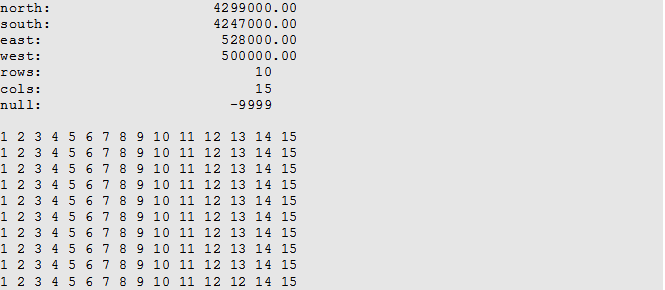
\includegraphics[scale=0.7]{1}
\end{figure}


The figure shown below is a DEM of size 5 x 5. The DEM is represented
as an array of integers representing elevation at a point. 

\begin{figure}[H]
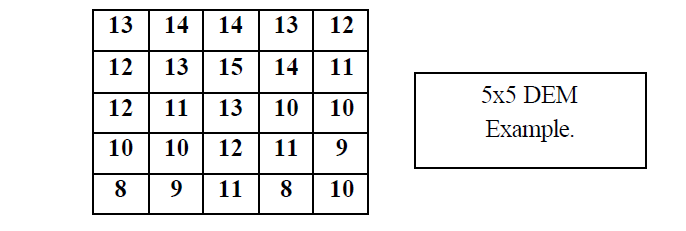
\includegraphics[scale=0.7]{10}\caption{DEM representation as 2D array of integers }


\end{figure}


The DEM ASCII file can be generated using FM2D or spectral synthesis
algorithm.

Fractional Brownian motion (FM2D) and Spectral Synthesis (SS) algorithms
is used to generate Digital Elevation Model, Both of these algorithms
are described in Saupe 1988 paper in great detail. FM2D is iterative
in nature whereas SS is sequential. So, FM2D takes a larger time compared
to SS to generate a DEM with same size and H (auto-correlation factor)
value. 

Few Digital Elevation models (DEMs): More the intensity of red (in
figure shown below) higher is the elevation. The figure shown below
are DEM obtained using FM2D algorithm. The 3rd image from left contains
gradient.

\begin{figure}[H]
\caption{DEM generated using FM2D algorithms }


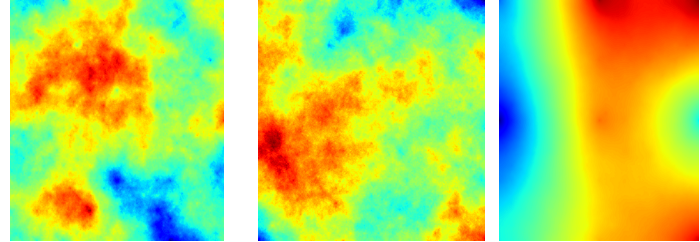
\includegraphics[scale=0.7]{11}
\end{figure}



\subsection{Slope in DEM}

For each cell, Slope calculates the maximum rate of change in value
from that cell to its neighbors. Basically, the maximum change in
elevation over the distance between the cell and its eight neighbors
identifies the steepest downhill descent from the cell. Conceptually,
the Slope function fits a plane to the z-values of a 3 x 3 cell neighborhood
around the processing or centered cell. 

The rate of change in the x direction for cell 'e' is calculated with
the algorithm: The neighbors are identified as letters from 'a' to
'i', with 'e' representing the cell for which the aspect is being
calculated.

\begin{figure}[H]
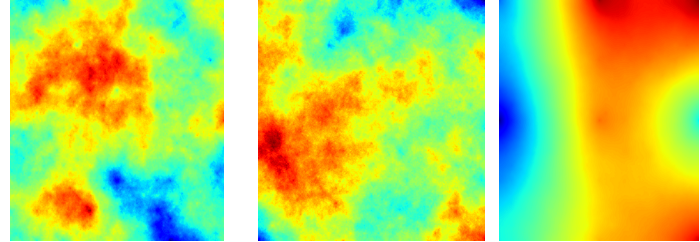
\includegraphics{11}\caption{3x3 window of cells}


\end{figure}


\[
[dz/dx=((c+2f+i)-(a+2d+g)/(8*x_{cellsize})]
\]


The rate of change in the y direction for cell 'e' is calculated with
the following algorithm:

\[
[dz/dy=((g+2h+i)-(a+2b+c)/(8*y_{cellsize})]
\]


\begin{figure}[H]
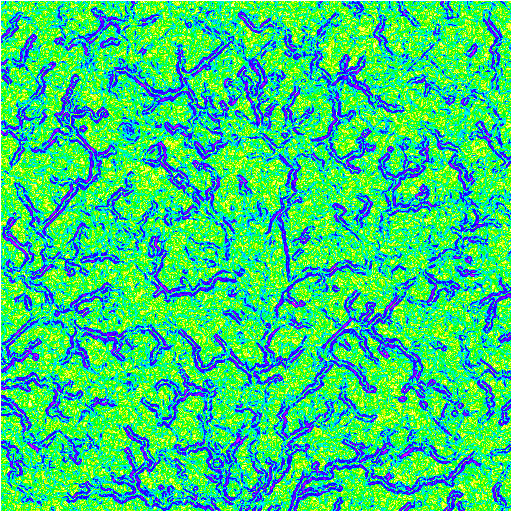
\includegraphics[scale=0.7]{12}\caption{3 Slope map of DEM calculated using GRASS GIS}


\end{figure}



\subsection{Aspect in DEM}

Aspect identifies the down slope direction of the maximum rate of
change in value from each cell to its neighbors. Aspect can be thought
of as the slope direction. The values of the output raster will be
the compass direction of the aspect.

A moving 3 x 3 window visits each cell in the input raster and for
each cell in the center of the window, an aspect value is calculated
using an algorithm that incorporates the values of the cell's eight
neighbors. The cells are identified as letters 'a' to 'i', with 'e'
representing the cell for which the aspect is being calculated.

The rate of change in the x direction for cell 'e' is calculated with
the following algorithm:

\[
[dz/dx=((c+2f+i)-(a+2d+g)/(8*x_{cellsize})]
\]


The rate of change in the y direction for cell 'e' is calculated with
the following algorithm:

\[
[dz/dy=((g+2h+i)-(a+2b+c)/(8*y_{cellsize})]
\]


Taking the rate of change in both the x and y direction for cell 'e',
aspect is calculated using: 

\[
[aspect=57.29578*atan([dz/dy],-[dz/dx])]
\]


The aspect value is then converted to compass direction values (0\textendash{}360
degrees), according to the following rule: 

\quad{}\quad{}\quad{}\quad{}\quad{}\quad{}\quad{}\quad{}\quad{}\quad{}\quad{}if
aspect < 0 

\quad{}\quad{}\quad{}\quad{}\quad{}\quad{}\quad{}\quad{}\quad{}\quad{}\quad{}\quad{}\quad{}cell
= 90.0 - aspect

\quad{}\quad{}\quad{}\quad{}\quad{}\quad{}\quad{}\quad{}\quad{}\quad{}\quad{}else
if aspect > 90.0

\quad{}\quad{}\quad{}\quad{}\quad{}\quad{}\quad{}\quad{}\quad{}\quad{}\quad{}\quad{}\quad{}cell
= 360.0 - aspect + 90.0

\quad{}\quad{}\quad{}\quad{}\quad{}\quad{}\quad{}\quad{}\quad{}\quad{}\quad{}else
cell = 90.0 - aspect 

\begin{figure}[H]


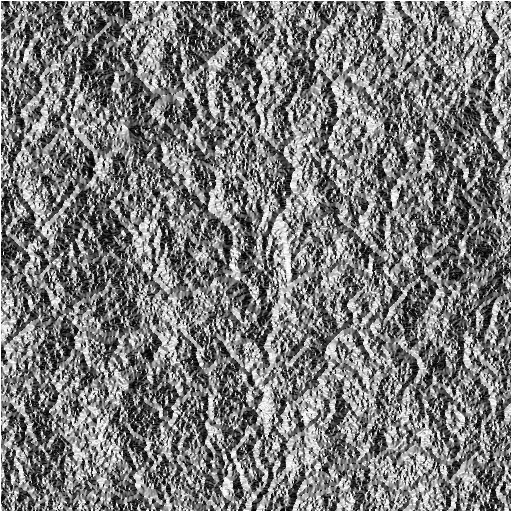
\includegraphics[scale=0.7]{13}\caption{Aspect map of DEM Calculated using GRASS GIS}


\end{figure}



\subsection{Decision tree}

A decision tree is a decision support tool that uses a tree-like graph
or model of decisions and their possible consequences. We create a
decision tree from the input training data. The training data contains
a DEM, land-cover class classification and river presence and absence
information. From River presence and absence algorithm we get the
river distance matrix. The leaf nodes in decision tree represent the
land-cover class. We query in decision tree just like a binary search
tree. We use this decision tree to assign land-cover class values
to synthetic landscape which in turn is used to assign suitability
values to each and every pixel. 

\begin{figure}[H]


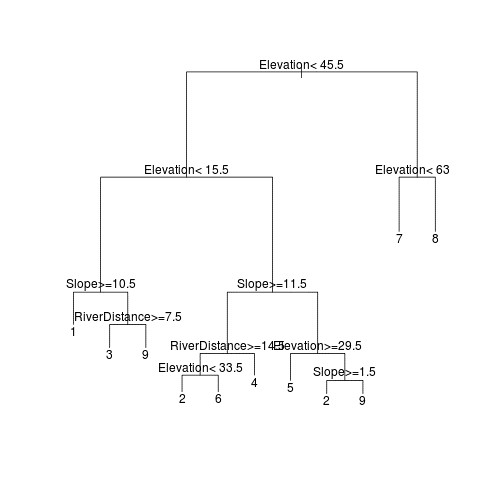
\includegraphics[scale=0.8]{14}\caption{Decision tree generated from training data}


\end{figure}



\subsection{Flow Direction (Hydrologic)}

Water flows in the direction of the steepest downhill gradient.

{\Large{D8 Algorithm (For 3x3 window)}}{\Large \par}

Every pixel is potentially surrounded by eight neighboring pixels.
The slope in each of these eight directions may be calculated by taking
the difference in elevation indicated by the DEM value at each of
these eight neighboring locations and the value at the pixel being
examined. This difference in elevation is then divided by the center-to-center
distance between these pixels (this distance will be the cell size
in the cardinal directions and the cell-size \texttimes{} $\sqrt{2}$
in each of the diagonal directions. The direction that yields the
steepest downhill slope is the inferred direction of water flow. (This
basic algorithm is sometimes referred to as the D8 method.)

Consider the following 3x3 DEM with a horizontal resolution of 30
meters and reported in vertical units of meters:

\begin{figure}[H]


\caption{3x3 window of a DEM}



\includegraphics[scale=0.7]{15}
\end{figure}


The figure shown below is a flow direction map using D8 flow algorithm
obtained using GRASS GIS.

\begin{figure}[H]
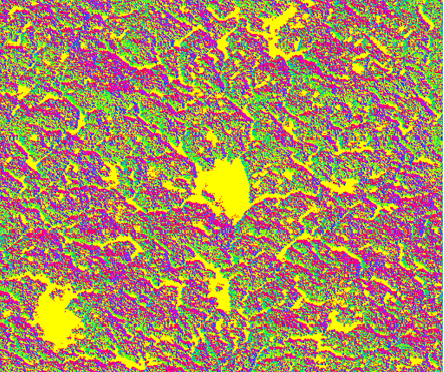
\includegraphics[scale=0.7]{8}\caption{Flow direction map of a DEM calculated using GRASS GIS}


\end{figure}



\subsection{Flow Accumulation (Hydrologic)}

Water accumulates along the flow paths dictated by the topography
and defined earlier as the flow direction. Using the flow directions
determined earlier, flow accumulation at a given location is determined
by following two rules:
\begin{enumerate}
\item If the pixel has no neighboring pixels draining to it, a value of
\textquotedblleft{}1\textquotedblright{} is assigned.
\item If the pixel drainage from neighboring pixels, it is assigned the
value of \textquotedblleft{}1\textquotedblright{} plus the sum of
the flow accumulation draining from each of the neighboring pixels.
\end{enumerate}
Rules 1 and 2 are repeated across the entire DEM.

Figure shown below is the flow accumulation map obtained using GRASS
GIS on a DEM. 

\begin{figure}[H]
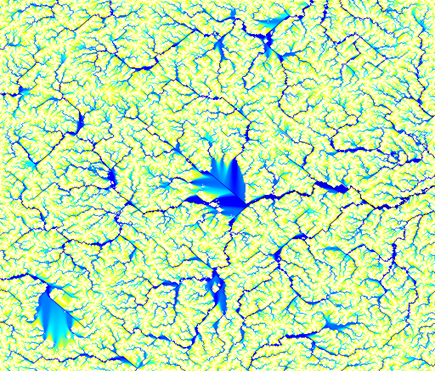
\includegraphics[scale=0.7]{7}

\caption{Flow accumulation map of a DEM calculated using GRASS GIS}


\end{figure}



\subsection{Erosion Modelling }

Erosion is the process by which soil and rock are removed from the
Earth's surface by natural processes such as wind or water flow, and
then transported and deposited in other locations. We carry out iterative
erosion modelling once we get the flow accumulation map. It is an
iterative process repeated by no of times specified by user. Once
we erode DEM then again hydrological modelling (flow direction and
flow accumulation) is performed followed by erosion modelling. This
process repeats itself the no of times specified by user.

Figures shown below is a DEM with and without erosion.

\begin{figure}[H]
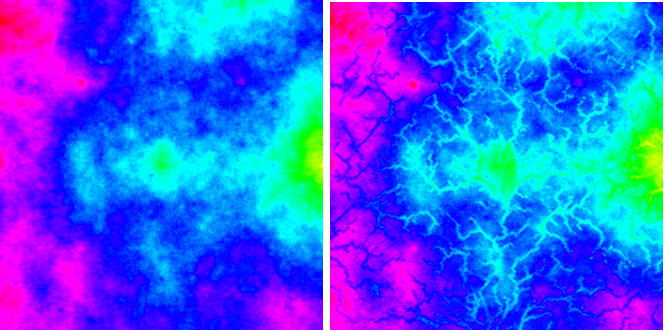
\includegraphics[scale=0.7]{6}\caption{DEM with (Right) and without (Left) erosion}


\end{figure}



\subsection{GRASS GIS}

GRASS GIS (Geographic Resources Analysis Support System) is a free,
open source geographical information system (GIS) capable of handling
raster, topological vector, image processing, and graphic data. We
write python script to use GRASS GIS functions to carry out hydrological
modelling, finding least cost path.


\subsection{Algorithm used to generate and place the agricultural patch onto
map}
\begin{itemize}
\item Generate a continuous 'suitability map' to guide placement. Areas
which match the rules for existing agriculture will have suitability
100\%. Other pixels should be labelled according to simple rules e.g.,
'slope < 20\%, elevation < x, moisture > y' and weighted by the current
land-cover. 
\item Threshold this suitability map at a desired percentage (e.g., 'we
want to end up with 70\% of the landscape covered in agriculture')
to discover the minimum suitability level to tolerate. i.e., if 70\%
of landscape pixels are above 32\% suitability, make this the threshold.
\item Generate the first patch - first, Get a min area, max area, and aspect
ratio from the user. Generate a grid of pixel row- column coordinates
for a shape of that aspect ratio and required area - e.g., 0,0 to
9,9. For the first block, this could be the mean area. Subsequent
blocks will only ever get smaller, so it could be the max. We choose
maximum. 
\item Rotate the feature by a random quantity, and recalculate the coordinates
of the pixels.
\item Find a highly suitable pixel in the map, and get its row and column
coordinate, r and c. After a few patches have been created, the algorithm
should look for suitable pixels close to other patches, to mimic spread.
\item Translate the rotated feature to this location by adding r and c to
each pixel
\item Investigate whether each pixel of the feature now lies in a suitable
location. Rules for removing that pixel include 'overlaps an existing
patch', 'on unsuitable habitat' and, optionally, if inter-patch strips
are required ' <2 pixels from an existing patch) 
\item Count the pixels that remain. If these are less than the specified
minimum area, don't keep this patch. If it's big enough, then give
this patch a unique ID, (by labelling all the pixels in this or a
separate 'patch map' and record its area, perimeter, state etc in
the patch list.
\item If an adjacency matrix is being maintained, update the cells which
tell us about all the neighbors of this patch.
\item Calculate the new area covered - if it doesn't meet the stopping threshold,
continue to create and lay down patches. 
\end{itemize}
\newpage{}


\section{Methodology }

The flow chart shown below describe the control flow within program.

\begin{figure}[H]
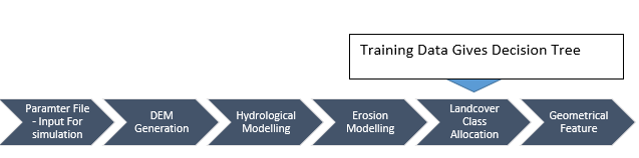
\includegraphics[scale=0.45]{5}\caption{Program Control Flow}


\end{figure}


Following steps describe the methodology followed:


\subsection{Input from parameter File}

User specify the simulation parameter in a parameter file. The program
reads the parameter from parameter file and then it starts landscape
simulation.


\subsection{Generation of Digital Elevation Model (DEM)}

A DEM is generated either by using Fractional Brownian motion with
midpoint displacement (midpointfM2D) or Spectral Synthesis (SS) method.
A set of DEMs are generated which are then linearly combined using
a weighted ratio specified in parameter file by the user. The DEM
generation consists of a set of parameter specified by user ,such
as a list of H (spatial autocorrelation) values, list of H weights,
list of seed values for random number generator, choice of method
used to generate DEM, size of DEM, gradient as true or false in case
of midpointfM2D.The parameter file is described in appendix. At the
end of this step we get a DEM which is a combination of DEM\textquoteright{}s
generated for given parameters.

DEM = (DEM1{*}H\_wt1) + (DEM2{*}H\_wt2) + \ldots{}+ (DEMn{*}H\_wtn)


\subsection{Hydrological Modelling and Erosion}

We carry out iterative hydrological modelling using GRASS GIS followed
by Erosion modelling. This process is repeated many times. The value
of counter in parameter file controls the number of iterations.


\subsection{Generation of decision tree for land-cover classification}

To assign land cover class to the synthetic DEM, we generate a decision
tree based on an input elevation map, land-cover map for the elevation
map and river presence/absence information for each and every pixel.
Using the elevation map, we calculate slope and aspect map. From river
presence/absence map, we get city block distance for each and every
pixel. Based on the information (elevation, slope, aspect, river distance,
land-cover class), we get a decision tree using rpart command in rpy
python library.


\subsection{Land-cover class mapping}

Using the decision tree, we assign the land-cover class to each and
every pixel of synthetic DEM generated in previous steps by first
calculation the slope, aspect, and distance from river for synthetic
DEM. 


\subsection{Generation of geometrical Features}

Once we assign the land-cover classes to each and every pixel, we
generate an agricultural suitability map. The suitability is assigned
based on some observation and common sense. Once we assign the suitability
values then we placed the agricultural patches (agricultural fields
of a specified aspect ratio, min area and maximum area) until we cover
specified part/fraction (fraction of area to be covered is supplied
by the user) of the map. After placing all the patches we carry out
patch labelling i.e. to assign unique ID to each patch. The algorithm
is described in the chapter 3, section 3.9. Once we get all the patches
we treat them as a graph. We try to connect patches using least cost
path. After that some patches can be converted to urban settlements.

\newpage{}


\section{Input Parameter File and It\textquoteright{}s Description}


\subsection{Input Parameter file}

The content of parameter file looks like this: 

\begin{figure}[H]
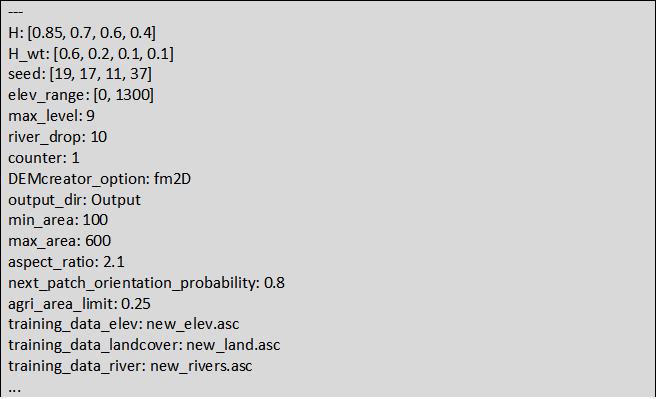
\includegraphics[scale=0.7]{4}\caption{Parameter File}


\end{figure}



\subsection{Parameter File Description }

\begin{table}
\caption{Parameter File Description}


\begin{tabular}{|c|c|}
\hline 
\multicolumn{1}{|c|}{{\tiny{General parameters}}} & \multirow{1}{*}{}\tabularnewline
\hline 
{\tiny{Output\_dir}} & \multicolumn{1}{c|}{{\tiny{The directory where output results (output images and files)
will be saved. Data-type: String }}}\tabularnewline
\hline 
{\tiny{H }} & \multirow{1}{*}{{\tiny{List of auto-correlation values }}}\tabularnewline
\hline 
{\tiny{H\_wt}} & {\tiny{List of weight for each correlation values specified in H list.
Data-type: {[}float, float, \ldots{}{]}}}\tabularnewline
\hline 
{\tiny{seed}} & {\tiny{List of values(ints preferably prime no\textquoteright{}s)
to be used as a seed for random number generator. Data-type: {[}int,
int, \ldots{}{]} }}\tabularnewline
\hline 
{\tiny{elev\_range}} & {\tiny{Range of elevation in DEM{[}min elevation, max elevation{]}
Data-type: {[}float, float{]} }}\tabularnewline
\hline 
{\tiny{max\_level }} & {\tiny{Size of the DEM grid 2\textasciicircum{}(max\_level) .Data-type:
int }}\tabularnewline
\hline 
{\tiny{river\_drop}} & {\tiny{Maximum extent of erosion, a fraction of this value is subtracted
from the DEM based on river distance. Data-type: float }}\tabularnewline
\hline 
{\tiny{counter}} & {\tiny{No of iteration of DEM erosion to be performed. Data-type:
int }}\tabularnewline
\hline 
{\tiny{DEMcreator\_option}} & {\tiny{Choice of the Algorithm used to generate DEM fm2D or SS Parameters
related to Decision tree module }}\tabularnewline
\hline 
{\tiny{training\_data\_elev }} & {\tiny{Name of the training data file in which elevation data is kept.
Data-type: String }}\tabularnewline
\hline 
{\tiny{training\_data\_landcover }} & {\tiny{Name of the training data file in which Landcover data is kept.
Data-type: String }}\tabularnewline
\hline 
{\tiny{training\_data\_river }} & {\tiny{Name of the training data file in which River presence/absence
data is kept. Data-type: String}}\tabularnewline
\hline 
{\tiny{min\_area }} & {\tiny{Minimum area of the fields allowed. Data-type : integer }}\tabularnewline
\hline 
{\tiny{max\_area}} & {\tiny{Maximum area of the field allowed. Data-type: integer }}\tabularnewline
\hline 
{\tiny{aspect\_ratio }} & {\tiny{Ratio of width to the height of the fields(rectangle). Data-type:
float }}\tabularnewline
\hline 
{\tiny{next\_patch\_orientation\_pr}} & {\tiny{Probability of next patch having the same orientation as the
previous patch placed. Data-type: float , Domain: 0 - 1 }}\tabularnewline
\hline 
{\tiny{agri\_area\_limit }} & {\tiny{Fraction of area in the grid to be covered by agricultural
patches. Data-type: float , Domain: 0 - 0.99}}\tabularnewline
\hline 
\end{tabular}
\end{table}


\newpage{}


\section{Conclusion}

We start with a parameter file and carry out landscape simulations.
We get the following outputs;
\begin{enumerate}
\item DEM with and without Erosion
\item Flow Accumulation Map 
\item Land-cover classification Map 
\item Geometrical Feature map 
\end{enumerate}
We have discussed the algorithm used to get the above layers in previous
chapters. The next chapter discusses about the future enhancements
in the project. Shown below is Land-cover classification map obtained
from decision tree and agricultural patch map.

\begin{figure}[H]
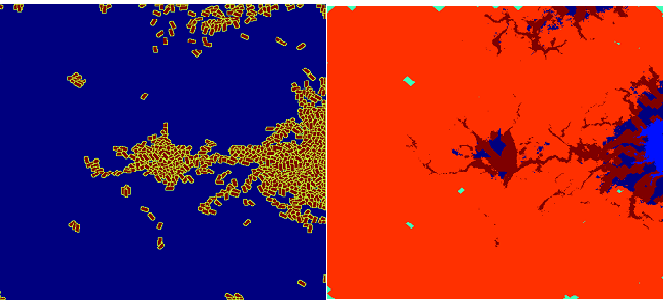
\includegraphics[scale=0.7]{3}

\caption{Agricultural patch map (left) land-cover classification map (right)}


\end{figure}


The DEM layer, flow accumulations layers were shown in previous chapters.
Currently the hydrological modelling is carried out using GRASS GIS.
We used Scotland training data to produce the synthetic landscapes.
\newpage{}


\section{Future work}


\subsection{GUI Interface}

In future a GUI Interface can be added to make it more convenient
to use.


\subsection{Improvement in Erosion Modelling}

More realistic erosion modelling algorithm can be incorporated to
make the DEM more realistic. Better the erosion modelling algorithm
better is the quality of DEM.


\subsection{Improvement in Patch Connectivity}

We use least cost path to connect cluster (set of patches which are
close to each other) of patches. We can treat patches as set of nodes
in a graph and then we can connect them using least cost path. Some
patches can be converted to urban features based on suitability rule.
Patches can be combined based upon requirements. Patches can even
be more fragmented. The figure shown below treat each patch as a node
and connect them using least cost path. The figure is included just
to illustrate the idea.

\begin{figure}[H]
\caption{Connectivity Map}
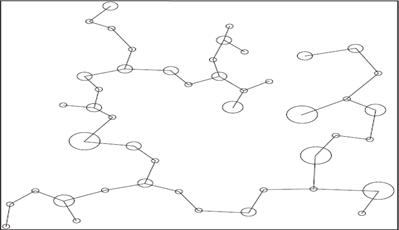
\includegraphics{2}

\end{figure}
\newpage{}


\section{Appendix }

{\Large{Software and Packages Required }}{\Large \par}

\medskip{}


Following software and packages need to be installed on Linux-Ubuntu
before running the grass script
\begin{enumerate}
\begin{spacing}{0.5}
\item Grass \end{spacing}

\begin{singlespace}
\item Python\end{singlespace}
\end{enumerate}
\begin{itemize}
\begin{spacing}{0.5}
\item numpy \end{spacing}

\begin{singlespace}
\item scipy 
\item pylab 
\item rpy 
\item yaml\end{singlespace}

\end{itemize}
\begin{singlespace}
RunMe.sh contain executable shell script code which will automatically
Install the given packages and software\textquoteright{}s.
\end{singlespace}

To run the RunMe.sh file 

--> Select the file -> press enter--> click on Execute

OR

Open the terminal, go to the directory in which RunMe.sh file is placed
using cd (change directory) command. Type \textquotedbl{}sh RunMe.sh\textquotedbl{}
and press enter.

\medskip{}


{*}{*}{*}{*}{*}{*}{*}{*}{*}{*}{*}{*}{*}{*}{*}{*}{*}{*}{*}{*}{*}{*}{*}{*}{*}{*}{*}{*}After
Installation{*}{*}{*}{*}{*}{*}{*}{*}{*}{*}{*}{*}{*}{*}{*}{*}{*}{*}{*}{*}{*}{*}{*}{*}{*}
\begin{enumerate}
\item Specify the parameters for landscape simulation in parameters.yaml
file in source code directory.
\item Now to run the simulation code, go to source code directory using
cd command in terminal and type \textquotedbl{}python main.py\textquotedbl{}
(without quotes) and press enter. 
\end{enumerate}
\newpage{}
\begin{thebibliography}{10}
\bibitem{key-1}Burrough, P. A. and McDonell, R.A., 1998. Principles
of Geographical Information Systems (Oxford University Press, New
York), p. 190.

\bibitem{key-2}Emilio Rafael D.-V., Manuel Francisco M.-P., Pedro
�.-�. (2009) Use of simulated and real data to identify heterogeneity
domains in scale-divergent forest landscapes. For. Ecol. Manage. 258:2490\textendash{}2500

\bibitem{key-3}Gardner R. H. (1999) RULE: map generation and a spatial
analysis program. In: J.M. K. andR.H. G. (eds), Landscape Ecological
Analysis: Issues and Applications. Springer, New York, pp. 280\textendash{}303

\bibitem{key-4}Gardner R. H., Urban D. L. (2007) Neutral models for
testing landscape hypotheses. Landscape Ecol. 22(1):15-29

\bibitem{key-5}Hargrove W. W., Hoffman F. M., Schwartz P. M. (2002)
A fractal landscape realizer for generating synthetic maps. Conserv.
Ecol. 6(1)

\bibitem{key-6}Keitt T. H. (2000) Spectral representation of neutral
landscapes. Landscape Ecol. 15(5):479-494

\bibitem{key-7}Li X., He H. S., Bu R. et al (2005) The adequacy of
different landscape metrics for various landscape patterns. Pattern
Recognition 38(12):2626-2638

\bibitem{key-8}Li X., He H. S., Wang X., Bu R., Hu Y., Chang Y. (2004)
Evaluating the effectiveness of neutral landscape models to represent
a real landscape. Landscape Urban Plann. 69(1):137-148

\bibitem{key-9}Riitters K. H., Vogt P., Soille P., Kozak J., Estreguil
C. (2007) Neutral model analysis of landscape patterns from mathematical
morphology. Landscape Ecol. 22(7):1033-1043

\bibitem{key-10}Saupe D. (1988) Algorithms for random fractals. In:
Peitgen H. O. andSaupe D. (eds), The science of fractal images. Springer-Verlag,
New York, pp. 71-113

\bibitem{key-12}Saura S., Mart\textasciiacute{}�nez-Mill�n J. (2000)
Landscape patterns simulation with a modified random clusters method.
Landscape Ecol. 15(7):661\textendash{}678

\bibitem{key-13}Shen W., Darrel Jenerette G., Wu J., H. Gardner R.
(2004) Evaluating empirical scaling relations of pattern metrics with
simulated landscapes. Ecography 27(4):459-469

\bibitem{key-14}Walters S. (2007) Modeling scale-dependent landscape
pattern, dispersal, and connectivity from the perspective of the organism.
Landscape Ecol. 22(6):867-881

\bibitem{key-15}Wang Q., Malanson G. P. (2008) Neutral Landscapes:
Bases for Exploration in Landscape Ecology. Geography Compass 2(2):319-339

\bibitem{key-16}http://softwright.com/dem.html

\bibitem{key-17}http://grass.osgeo.org/grass64/manuals/r.in.ascii.html

\bibitem{key-1}http://geography.about.com/od/physicalgeography/a/landscapeecolog.htm\end{thebibliography}

\end{document}
